\chapter{Construction}
\label{chapter:construction}
This chapter describes the implementation of the applications studied in the
experiments. The experiments and their results are described in
\ref{chapter:experiments}. First the common idea behind the video filtering
applications is explained and the filters used are described. After that the
PREESM and OpenEM filter applications are introduced and last the PSE model of
the OpenEM filter application is explained. This chapter is focused on the
design and implementation of the applications.

\section{Filter Application}
\label{sec:filterapp}
The objective of this thesis is to study the suitability of OpenEM framework
for stream processing. Today many different types of data can be streamed, for
example audio and video. Video was chosen to be the type of the streams used in
the experiments because there are many known image processing algorithms to use
as the basis for the study and there are many applications for video stream
processing in the context of industrial internet. TODO: ????

Three requirements for the workload applications were specified to guide the
design. The requirements are presented in the following list.

\begin{enumerate}
    \item{Variable input bitrates}
    \item{Comparability the PREESM and OpenEM applications}
    \item{Highly analyzable}
\end{enumerate}

\textbf{Variable input bitrates} were required of the workload applications to
make it possible to study the performance of the OpenEM framework in processing
dynamic workloads. Varying the bitrates of the video stream inputs is simple as
the frame size of the stream is easy to change and it doesn't affect the
algorithms used in any unforeseeable way. \textbf{Comparability of the PREESM
and OpenEM applications} was required so the PREESM workload could be used as a
baseline implementation. Last requirement for the applications was that they
needed to be \textbf{highly analyzable} in order to enable the study of OpenEM
performance. An application satisfying these requirements was designed using the
PREESM sobel example at \cite{preesmtut} as the starting point and adding
another processing component to it. It is important to notice that the actual
performance of the filter application in its nominal video filtering task was
mostly disregarded. For example the data is copied to a new buffer in every
processing stage and the filter algorithms are not optimized for the specific
platform. Therefore comparing the performance of the implemented applications to
real world implementations of similar applications is not useful.

The idea for using sobel and gauss filters in the same application came from
the canny edge detector, which is briefly discussed in \ref{subsec:canny}. The
canny edge detector only provided ideas of what a realistic video processing
application does. The filters in the workload applications are executing
independently of each other on separate video streams unlike how they are
connected in the canny edge detector. After the introduction to edge detection
and the canny edge detector the filter components implemented in this thesis are
introduced in \ref{subsec:gauss} introducing the gaussian filter and
\ref{subsec:sobel} providing an overview on the sobel filter.\\

TODO: improve intro and find sources for claims. wikipedia on edge detection has
about the same stuff as above.

\subsection{Canny edge detector}
\label{subsec:canny}
Edge detection is an important tool in image processing and computer vision.
Many image processing and computer vision algorithms operate on detected edges.
There is a growing interest in the industry to use DSP platforms for edge
detection based algorithms.

In his 1986 paper John F. Canny \cite{canny1986computational} lays out the
mathematical criteria for successful edge detection and presents an algorithm,
which is suitable for implementation on DSP platforms and achieves decent edge
detection performance. The Canny Edge Detection consists of five steps
presented in the following list.

\begin{enumerate}
    \item{Noise reduction}
    \item{Finding the intensity gradient of the image}
    \item{Non-maximum supression}
    \item{Double tresholding}
    \item{Edge tracking by hysteresis}
\end{enumerate}

The noise reduction in step one can be implemented with gaussian filtering.
Finding the intensity gradient of the image in step two can be implemented using
a sobel filter. Gauss and sobel filters are implemented in the thesis
experiment. Gaussian filtering is discussed in \ref{subsec:gauss} and sobel
filtering in \ref{subsec:sobel}.  The rest of the steps are not implemented in
this thesis and thus are only briefly discussed here.

In the canny edge detector the image is first filtered with gaussian filter to
reduce the amount of noise in the image. Second the changes in the intensity in
the image are detected using an edge detection operator such as the sobel
operator. The third step improves the accuracy of the edge detection by
supressing all but the strongest responses to the detected edges, in practice
``thinning'' the edges. The fourth step classifies the edge pixels to three
classes separated by empirically determined threshold values. The pixels with
gradient value above the high threshold are marked strong pixels and the pixels
with gradient value below the low threshold are supressed. In the fifth step the
remaining weak pixels with gradient values below the high threshold are
preserved or supressed according to the presence of strong pixels in their
neighborhood. Detailed description of the algorithm is presented in the original
paper by Canny \cite{canny1986computational}, information about implementing a
canny edge detector is available in \cite{gonzalez2008digital} and comparison of
its performace to other edge detectors can be found in \cite{maini2009study}.

\subsection{Gaussian filter}
\label{subsec:gauss}
Gaussian filtering is used for multiple purposes in digital image processing.
In the canny edge detector the gaussian filter is used to reduce noise in the
processed images. The gaussian filter works by convolving a gaussian function
with the input signal. Gaussian function is non-zero everywhere which means it
would theoretically require an infinite convolution window. Since the function
decays rapidly it is often reasonable to truncate the function and use small
windows. \cite{gonzalez2008digital} In the thesis experiment a kernel size of
5x5 is used.

In practice every pixel in the filtered image has an intensity value computed
by taking a weighted average of the neighboring pixels in the input image. The
weights are precalculated from the gaussian function, giving the highest weight
to the pixel in the center of the window. The gaussian filter displayed in
figure \ref{fig:gaussmat} was calculated with $\sigma$ = 1.3. The filtered
image has a smoothed appearance compared to the original image.

\begin{figure}
    \begin{displaymath}
        B = \frac{1}{159}\begin{bmatrix}
             2 & 4 & 5 & 4 & 2 \\
             4 & 9 & 12 & 9 & 4 \\
             5 & 12 & 15 & 12 & 5 \\
             4 & 9 & 12 & 9 & 4 \\
             2 & 4 & 5 & 4 & 2 \\
        \end{bmatrix} \ast A
    \end{displaymath}
    \caption{The gaussian filter used in the filter applications. The
    convolution operation is denoted by the asterisk.}
    \label{fig:gaussmat}
\end{figure}

\subsection{Sobel filter}
\label{subsec:sobel}
The actual edge detection in the canny edge detector begins with applying the
sobel operator to the input image. The sobel operator is a discrete
differentiation operator. It consists of two 3x3 kernels which are convolved
with the image to approximate the derivatives. The two kernels represent
horizontal and vertical changes. At each point in the image the resulting
gradient approximations are combined giving an approximate gradient magnitude.
\cite{gonzalez2008digital} The convolution operations are presented in figure
\ref{fig:sobelmat}.

\begin{figure}
    \begin{displaymath}
        G_{x} = \begin{bmatrix}
            -1 & 0 & +1 \\
            -2 & 0 & +2 \\
            -1 & 0 & +1 \\
        \end{bmatrix} \ast A
    \end{displaymath}

    \begin{displaymath}
        G_{y} = \begin{bmatrix}
            -1 & -2 & -1 \\
            0 & 0 & 0 \\
            +1 & +2 & +1 \\
        \end{bmatrix} \ast A
    \end{displaymath}
    \caption{The Sobel Kernels used in the application to compute the gradient
    approximation. The asterisk denotes the convolution operation.}
    \label{fig:sobelmat}
\end{figure}

\section{PREESM Filter Application}
\label{sec:preesmapp}
An actor network is constructed in PREESM that represents the video filter
application. The final PiSDF model of the PREESM video filter application is
presented in figure \ref{fig:preesm_actors}. The PREESM filter application is
adapted from the PREESM example at \cite{preesmtut} by adding another
processing path for the gaussian filter and making the necessary modifications
to the shared parts of the application.

\begin{figure}[h!]
    \begin{center}
        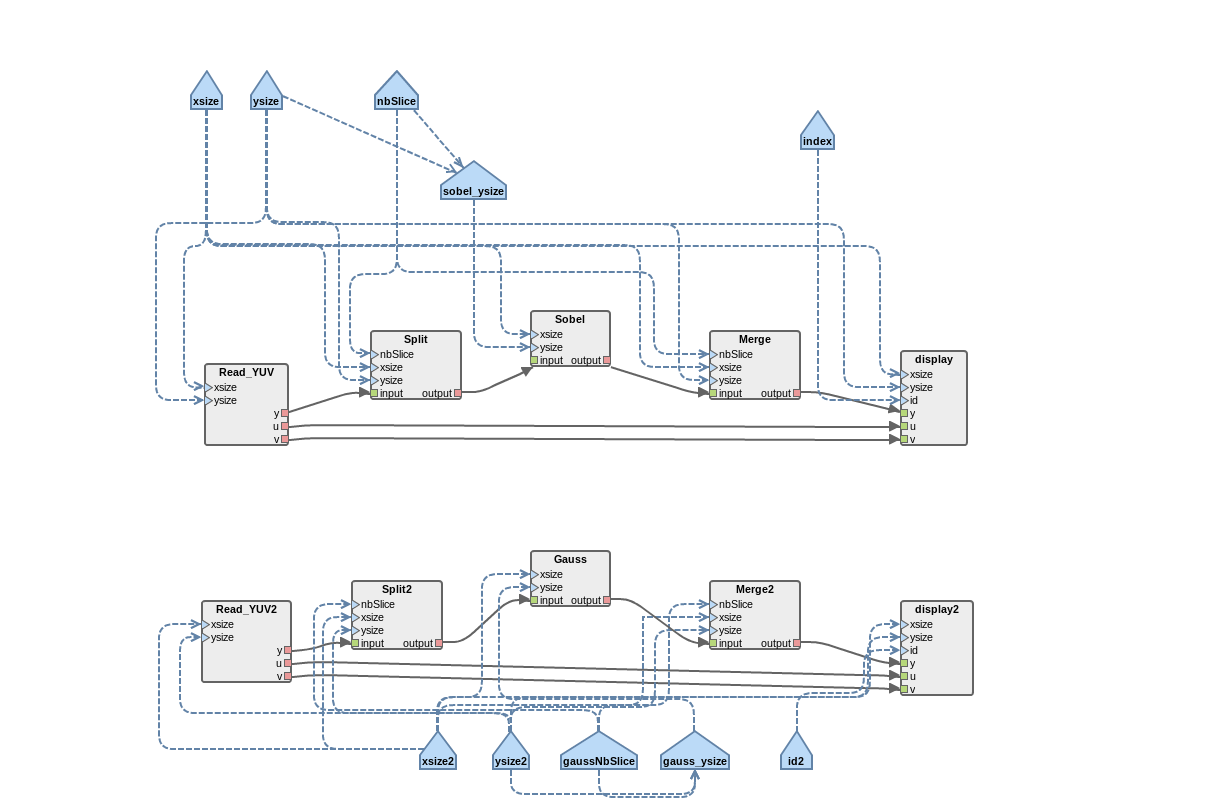
\includegraphics[width=0.99\textwidth]{images/preesm_diagram.png}
        \caption{The PiSDF graph of the PREESM filter application}
        \label{fig:preesm_actors}
    \end{center}
\end{figure}

\subsection{The Actor Model}
\label{subsec:actors}
To keep the model simple and the program well analyzable both of the processing
paths in the network are independent.

The first actor on both of the processing paths, the Read\_YUV and the
Read\_YUV actors in the figure \ref{fig:preesm_actors}, loads the video frames
from memory and passes them to splitting actors. The splitting actors split the
frames to a suitable number of splices to enable processing of the same video
stream on multiple cores. The filter actors, Sobel and Gauss actors in the
figure, follow the splitting actors. Partial frames filtered in the filter
actor are merged back to whole frames in the merge actors. The last actors on
both of the processing paths are dummy actors. The pentagons in the top and the
bottom of the figure represent the parameters of the application. The xsize,
ysize, xsize2 and ysize2 parameters specify the size of the input frames.
nbSlice and gaussNbSlice determine the numbers of slices the frames are split
to. The sobel\_ysize and gauss\_ysize are the heights of the slices after
splitting.

The first actors Read\_YUV and Read\_YUV2 call the \texttt{readYUV} function
defined in the PREESM example at \cite{preesmtut}. As I/O is not in the scope of
the experiments it is omitted from the application. The processing starts with
loading the frames from memory. In a real world application the frames would be
written in the memory for example with DMA by a packet processor processing a
stream of network packets. The \texttt{readYUV} function copies the Y component
of the input frame to the output address while the U and V components are
ignored. The U and V are omitted because the sobel and gauss actors only operate
on the Y channel. TODO: explain YUV format and how it's used here.

The split actor operates on the output of the Read\_YUV actor. The split actor
preprocesses the frame for the sobel and gauss actors. Since the sobel and gauss
filters involve convolution with 3x3 and 5x5 matrices respectively, they will
need to access image data outside the part of the image they are processing. To
enable parallel processing of a single frame on multiple cores, the frame is
split in to slices. These slices will also need to contain a bit of extra data
so that the filters can operate correctly. Black lines, or lines with the Y
value of 0 are added to the top and the bottom of the frame. One black line is
enough for the sobel frames but two black lines are needed for the gaussian
frames, corresponding to the filter kernel sizes.  With the black lines added
the frame is then copied to the output buffer one slice at a time. The slices
overlap each other for one or two lines again corresponding to the size of the
filter kernel.

The sobel actor calculates the convolution of the sobel kernels in presented in
\ref{fig:sobelmat} with the Y component of the input frame. The sobel actor is
copied as is from the PREESM example at \cite{preesmtut}. The convolution is
computed by looping over the pixels in the input frame, calculating the $G_{x}$
and $G_{y}$ components of the sobel operator in one line expressions and
combining them by taking the absolute values of $G_{x}$ and $G_{y}$ and dividing
the sum by eight. After looping over the image the actor sets the leftmost and
rightmost columns to 0.

The gauss actor operates similarly to the sobel actor but instead of one line
expressions the value of the filter function at each points is calculated by
looping over the neighboring pixels and multiplying the intensity values by the
corresponding weight from the gaussian kernel presented in \ref{fig:gaussmat}.
The Texas Instruments compiler transforms the innermost loops in a loop
optimization pass resulting in less branches in the executable code than the
multi-leveled loop structure would suggest. The weighted average is calculated
simply by division. Finally the leftmost and rightmost columns are set to 0 as
in the sobel actor.

The last actor processing the frame is the merge actor. The merge actor copies
the processed data from its input buffer to its output buffer, overlaying the
slices so that the output frame doesn't contain the extra lines created in the
split actor. Since there is no real I/O in the application, the merged frame is
not processed further. In a real world application the processed frame would be
copied for example to a network packet.

As there is no I/O the display actors don't do any computations. In the
experiments the display actor is used as the endpoint of the processing and it
starts the data export.

\subsection{The PREESM Schedule}
\label{subsec:preesmsched}

The scheduler in the PREESM framework is described in \ref{sec:preesmsched}.
The scheduler creates a block schedule from the actor model using user provided
estimates for the actor durations. To get reasonably accurate estimates, the
application was first scheduled with the default values and the actor durations
were measured on the target device. The resulting timings are presented in the
table \ref{tab:preesm_times}. The timings from the measurements were approximately
the same for all the actors except for the gauss actor. A gantt
chart representing the schedule created using the values in the table is
presented in figure \ref{fig:preesm_gantt}. The mutable parameters in the graph
\ref{fig:preesm_actors} affect the static memory allocations of the PREESM
application and the PREESM codegen workflow needs to be executed every time the
parameters are changed. Because of this the PREESM schedules of the different
measurement setups are slightly different.

\begin{table}
    \begin{center}
        \begin{tabular}{| c | c |}

            \hline
            Cycles & Actor \\ \hline
            600 & Gauss \\ \hline
            150 & Merge \\ \hline
            150 & Merge2 \\ \hline
            150 & Read\_YUV \\ \hline
            150 & Read\_YUV2 \\ \hline
            150 & Sobel \\ \hline
            150 & Split \\ \hline
            150 & Split2 \\ \hline
            1 & display \\ \hline
            1 & display2 \\ \hline
        \end{tabular}
        \caption{PREESM Actor Timings.}
        \label{tab:preesm_times}
    \end{center}
\end{table}

The PREESM framework doesn't support changing the timing of the implode and
explode operations which started affecting the schedule considerably with larger
frame sizes. The duration estimates used by PREESM for the implode and explode
operations are very short compared to durations of the actors measured from the
application. The explode operations for both streams are represented in the
gantt chart by the small time slices predecing gauss actors on cores 4 and 7.
The implode operation for gauss stream follows the gauss actor execution on core
7 and the implode operation of sobel stream follows the latter sobel actor on
core 5.

\begin{figure}[h!]
    \begin{center}
        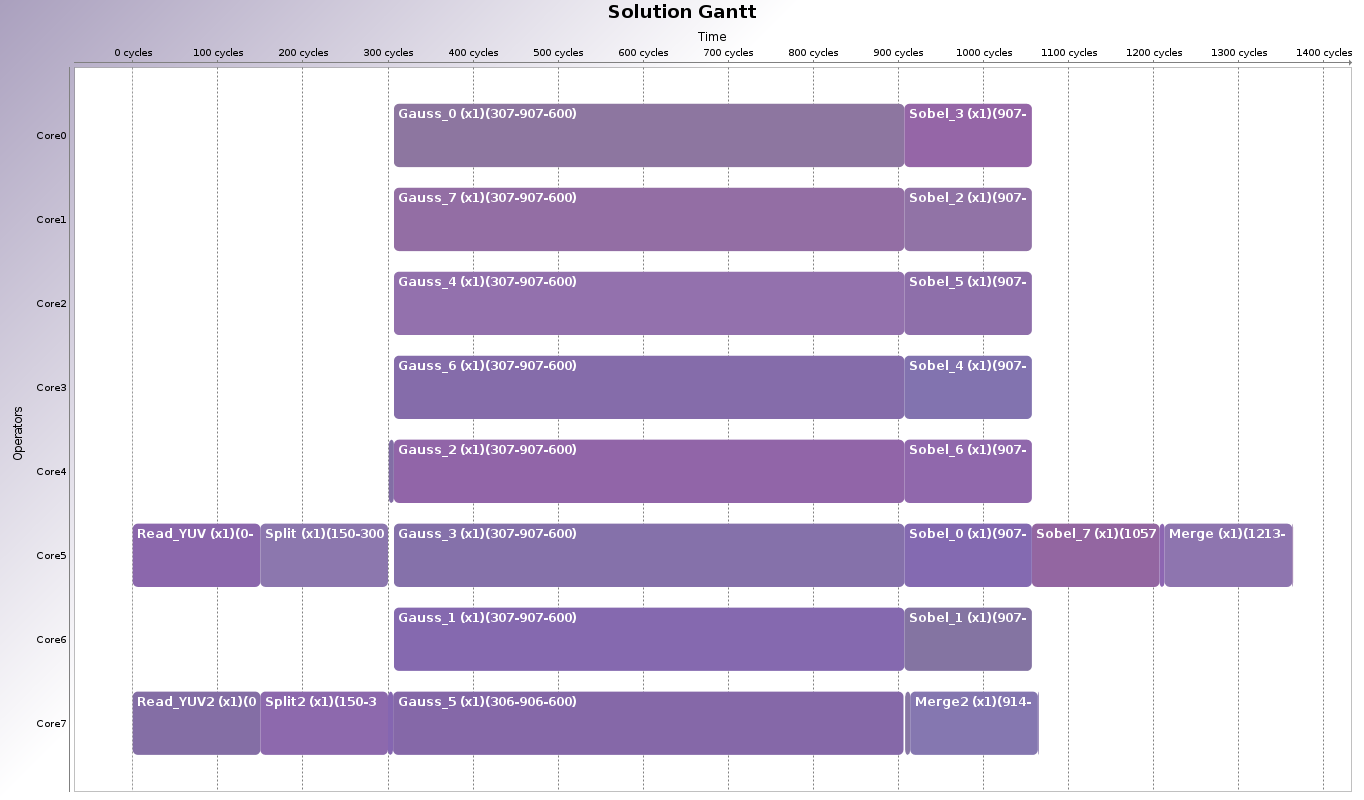
\includegraphics[width=0.99\textwidth]{images/gantt_preesm_cifcif.png}
        \caption{Gantt chart representing the schedule of a PREESM Filter
        Application.}
        \label{fig:preesm_gantt}
    \end{center}
\end{figure}

\section{OpenEM Filter Application}
\label{sec:oemapp}
The OpenEM implementation of the filter application was designed using the
PREESM filter application described in \ref{sec:preesmapp} as the starting
point. Specifically the OpenEM application has to process the frames in similar
manner so that only the scheduling policies between the two programming models
should differ. The high-level structure of the OpenEM filter application is
presented in the figure \ref{fig:openem_flow}. The application consists of two
atomic queues, a parallel queue and three execution objects. Each queue is
connected to only one execution object. In this text the queues are referred to
by the execution objects they are connected to, for example the atomic queue
connected to the merge eo will be referred to as the merge queue. The execution
runs in cycles. A new cycle is started every time a cycle finishes. There are
multiple cycles running in parallel, but since the read and merge EOs are
atomic, only filter EO is running on multiple cores in parallel.

The design principles introduced in the beginning of this chapter apply to the
OpenEM application as well. The OpenEM application was not designed for maximum
performance but to demonstrate the suitability of OpenEM as a platform for
stream processing applications. The performance of the application could be
improved in many ways, for example by minimizing the amount of redundant copying
of the frame slices and introducing parallelism to frame reading and merging.

\begin{figure}[h!]
    \begin{center}
        \usetikzlibrary{chains}

\begin{tikzpicture}[>=latex,node distance=0pt, scale=0.7, every node/.style={transform shape}]
    % the rectangular shape with vertical lines
    \node[rectangle split, rectangle split parts=6,
    draw, rectangle split horizontal,text height=0.5cm,text depth=0.5cm,inner sep=0pt, text width=0.0cm] (atomic1) {};
    \fill[white] ([xshift=-\pgflinewidth,yshift=-\pgflinewidth]atomic1.north west) rectangle ([xshift=-5pt,yshift=\pgflinewidth]atomic1.south);

    \node[draw,ellipse,right= 0pt of atomic1,minimum height=1.0cm,inner xsep=5pt] (readEO) {Read EO};

    \node at (5, 0)[rectangle split, rectangle split parts=6,
    draw, rectangle split horizontal,text height=0.5cm,text depth=0.5cm,inner sep=0pt, text width=0.0cm ] (parallel) {};
    \fill[white] ([xshift=-\pgflinewidth,yshift=-\pgflinewidth]parallel.north west) rectangle ([xshift=-5pt,yshift=\pgflinewidth]parallel.south);

    \node[draw,ellipse,right= 0pt of parallel,minimum height=1.0cm,inner xsep=5pt] (filterEO) {Filter EO};

    \node at (10, 0)[rectangle split, rectangle split parts=6,
    draw, rectangle split horizontal,text height=0.5cm,text depth=0.5cm,inner sep=0pt, text width=0.0cm] (atomic2) {};
    \fill[white] ([xshift=-\pgflinewidth,yshift=-\pgflinewidth]atomic2.north west) rectangle ([xshift=-5pt,yshift=\pgflinewidth]atomic2.south);

    \node[draw,ellipse,right= 0pt of atomic2,minimum height=1.0cm,inner xsep=5pt] (mergeEO) {Merge EO};

    % the arrows and labels
    \draw [->](readEO) to (parallel);
    \draw [->](filterEO) to (atomic2);
    \draw [->](mergeEO) .. controls (16,0) and (15, 2) .. (6, 2) .. controls (-2, 2) and (-3, 0) .. (atomic1);

    \node[align=center,below] at (atomic1.south) {Atomic Queue};
    \node[align=center,below] at (parallel.south) {Parallel Queue};
    \node[align=center,below] at (atomic2.south) {Atomic Queue};
\end{tikzpicture}

        \caption{The OpenEM filter application.}
        \label{fig:openem_flow}
    \end{center}
\end{figure}

The application execution starts with initializing the OpenEM framework and the
application data structures. The OpenEM initialization is explained in
\ref{subsec:ti_init_layer}. After the queues and the execution objects have been
initialized the application creates a number of initial events that are sent to
the the read queue. Once the events have been queued the application
synchronizes all cores and the actual execution starts.

The Read EO combines the functionality of the read and split actors of the
PREESM filter application presented in \ref{fig:preesm_actors}. A frame is read
from the input video memory and split in to a number of slices. The functions
called are exactly the same as in the PREESM application. The frame slices are
copied to event buffers of new events. The new events are then sent to the
filter queue. There is only one filter queue and one filter execution object.
The same execution object will compute either sobel or gauss filter on the
frame slice according to its type.

The PREESM application splits the frames into slices and processes the slices
separately before merging them back into one frame. Similar fork-join mechanism
was implemented in the OpenEM application. Event groups were first planned to be
used as the fork-join mechanism in the filter application but in the final
implementation a different, simpler mechanism was used. The TI implementation of
event groups lacks \texttt{em\_event\_group\_delete} function which makes it
necessary to reuse the existing event groups. The example applications which are
included in the NSN OpenEM distribution described in \ref{sec:emframework}
demonstrates the reuse of event groups, but it was estimated that the
programming overhead resulting from the reuse of the groups would be larger than
implementing the fork-join in a simpler manner. In the final implementation the
frames are accumulated simply in a merge buffer located in shared memory which
is referenced through queue context pointers. The bookkeeping for frame
completion is handled in the same location.

The filtered frame slices are accumulated in the merge buffer, which is accessed
through the merge queue context. The merge queue is atomic to avoid need for
synchronization between the cores. After a frame has been merged the merge EO
creates a new event which is sent to the read queue. The ratio of sobel filtered
frames to gauss filtered frames is always one to one.

\section{PSE Model of OpenEM Filter Application}
\label{sec:pse_model}
A PSE model of the OpenEM filter application was constructed. The OpenEM filter
application was modeled to identify the most important factors of performance of
the OpenEM framework. To fulfill the objective the application model had to be
kept simple but still capable of explaining runtime behavior. The construction
of the model is explained in this section. The PSE tool is described in chapter
\ref{chapter:pse}. The top-level software model is presented in the figure
\ref{fig:pse_application} and the hardware model in figure
\ref{fig:pse_hardware}.

\begin{figure}[h!]
    \begin{center}
        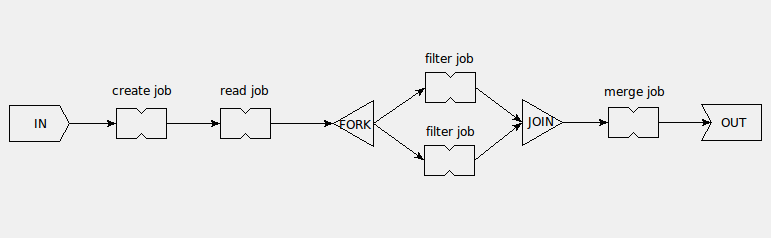
\includegraphics[width=0.99\textwidth]{images/pse_filterapp.png}
        \caption{The top-level PSE task graph of the OpenEM filter app PSE
        model.}
        \label{fig:pse_application}
    \end{center}
\end{figure}

The software model presented in figure \ref{fig:pse_application} has the same
structural elements as the OpenEM filter application described in section
\ref{sec:oemapp}. The most important distinction between the structure of the
OpenEM application and the PSE model is that the PSE model does not process
frames in cycles where a new frame is taken into processing every time another
frame finishes. Instead the application is loaded by generating work in a
simple workload model, which enqueues a new frame for processing periodically.
The nodes titled read job, filter job and merge job correspond to execution
objects in the filter application. The create job does not correspond to an EO
in the OpenEM application but a regular function called in the beginning of
processing each frame.

\begin{table}
    \begin{center}
        \begin{tabular}{| c | c | c |}
            \hline
            Quantity & Resource & Node \\ \hline
        \end{tabular}
        \caption{PSE software model resource usage.}
        \label{tab:pse_resources}
    \end{center}
\end{table}

\begin{figure}[h!]
    \begin{center}
        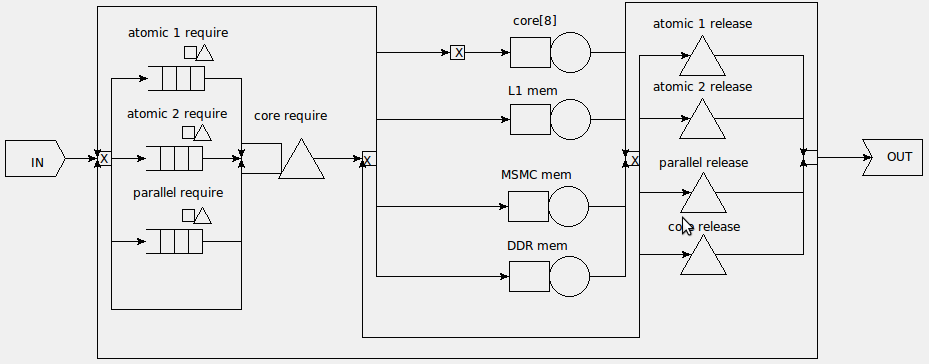
\includegraphics[width=0.99\textwidth]{images/pse_hardware.png}
        \caption{The PSE resource network of the OpenEM filter app PSE
        model.}
        \label{fig:pse_hardware}
    \end{center}
\end{figure}

The jobs in the application model use the hardware resources presented in figure
\ref{fig:pse_hardware}. The resource usage is controlled by the software
submodels and the usage quantities are based on measurements of the OpenEM
filter application. The resource usage is presented in table
\ref{tab:pse_resources}. The processing in each node of the software model
follows a simple approximation of the OpenEM filter application execution. First
the software model requests a queue resource to simulate queueing in the real
OpenEM application. There are one of each atomic queue resources and eight of
parallel queue resources. Once the process gets a queue resource it requests a
core resource. To this point no hardware delays have been accounted for in the
simulation. After getting a core token, the process proceeds to execution. As
the OpenEM scheduler doesn't support pre-emption, the core token can be held by
each EO for the full time of its execution. The delays of the software models
are approximated to be mostly caused by the memory except for the filtering
nodes where the computation of the filter is assumed to be limited by the cpu
speed. After the processing completes in each software node the hardware
resources are released in the release nodes.

In the simulation model the frame is only split to two slices due to the limited
forking capabilities of the PSE framework. This limits the potential for
parallelism especially with workloads that don't require a lot of processing in
the filter nodes. The effects of this and other simplifications to the
predictivity of the model are explored in the experiments.

\section{Instrumentation}
\label{sec:instrumentation}
To understand the behavior and performance of the applications their execution
needs to be measured. The measurements conducted in the experiments were based
on cycle counts. The TMS320C6678 exposes cycle counts on each core through two
registers, namely TSCL and TSCH which store the low 32 bits and the high 32 bits
of the cycle count respectively. Comparing the values of the TSCL register in
the beginning and the end of processing on each core gives accurate local
timings and would be enough for measuring the execution on single core. However
for accurate measurements of global cycles, the cycle offsets to the global
cycle count needed to be stored. The functionality for counting cycles was
included in the Texas Instruments OpenEM initialization and utilities code. The
cycle counts were stored in the DDR memory.

In the PREESM application the cycle counts were saved in the beginning and the
end of each user defined function of the application. In addition to this total
cycle count was measured in the \texttt{readYUV} function.

In the OpenEM application cycle counts were measured over the same functions as
in the PREESM application and in the beginning and in the end of each EO. The
latter measurements were carried out to get a better understanding of the OpenEM
runtime overhead.

The measurements were exported through the debug connection of the TMS320C6678
using I/O library provided by Texas Instruments.
